\newpage
\begin{chapterbox}
	\chapter{Direct numerical simulations of forced HIT field} \label{ch:chap4}
\end{chapterbox}
\thispagestyle{empty}
\vfill
\begin{courtesybox}
	Background image: ...
\end{courtesybox}
\AddToShipoutPictureBG*{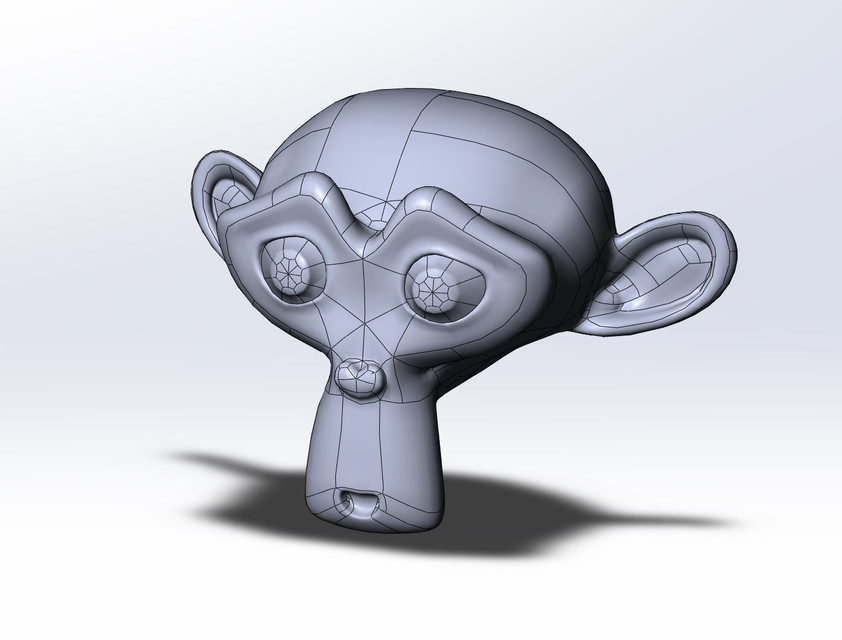
\includegraphics[height=\paperheight,trim=3cm 0 0 0cm]{Figures/chapterCovers/placeholder.jpg}}

\newpage
\thispagestyle{abstract}
\begin{abstractbox}
	\section*{Abstract}
	\lipsum[1-1]
\end{abstractbox}
\newpage
\section{Introduction}
\subsection{Motivation and goals}
\section{Simulation setup}
\section{Analysis setup}
\section{Results and discussion}
\subsection{Visualization}
\subsection{Trends of clustering timescales and magnitudes}
\subsection{Effects of combustion on particle clustering}
\subsection{Global temperature evolutions}
\subsection{Burnout times at various $\mathrm{Re}$ and $\phi$}
\subsection{Correlating spatial and combustion properties}
\subsubsection{Underlying trends in $\tau_\mathrm{b}^*$ vs. $V_\mathrm{norm}$}
\subsubsection{Time-averaging spatial properties}
\subsubsection{Significance of macroscale structures}
\section{Summary}